\section{Introduction}\label{sec:intro}

\begin{figure}[t]
\centering
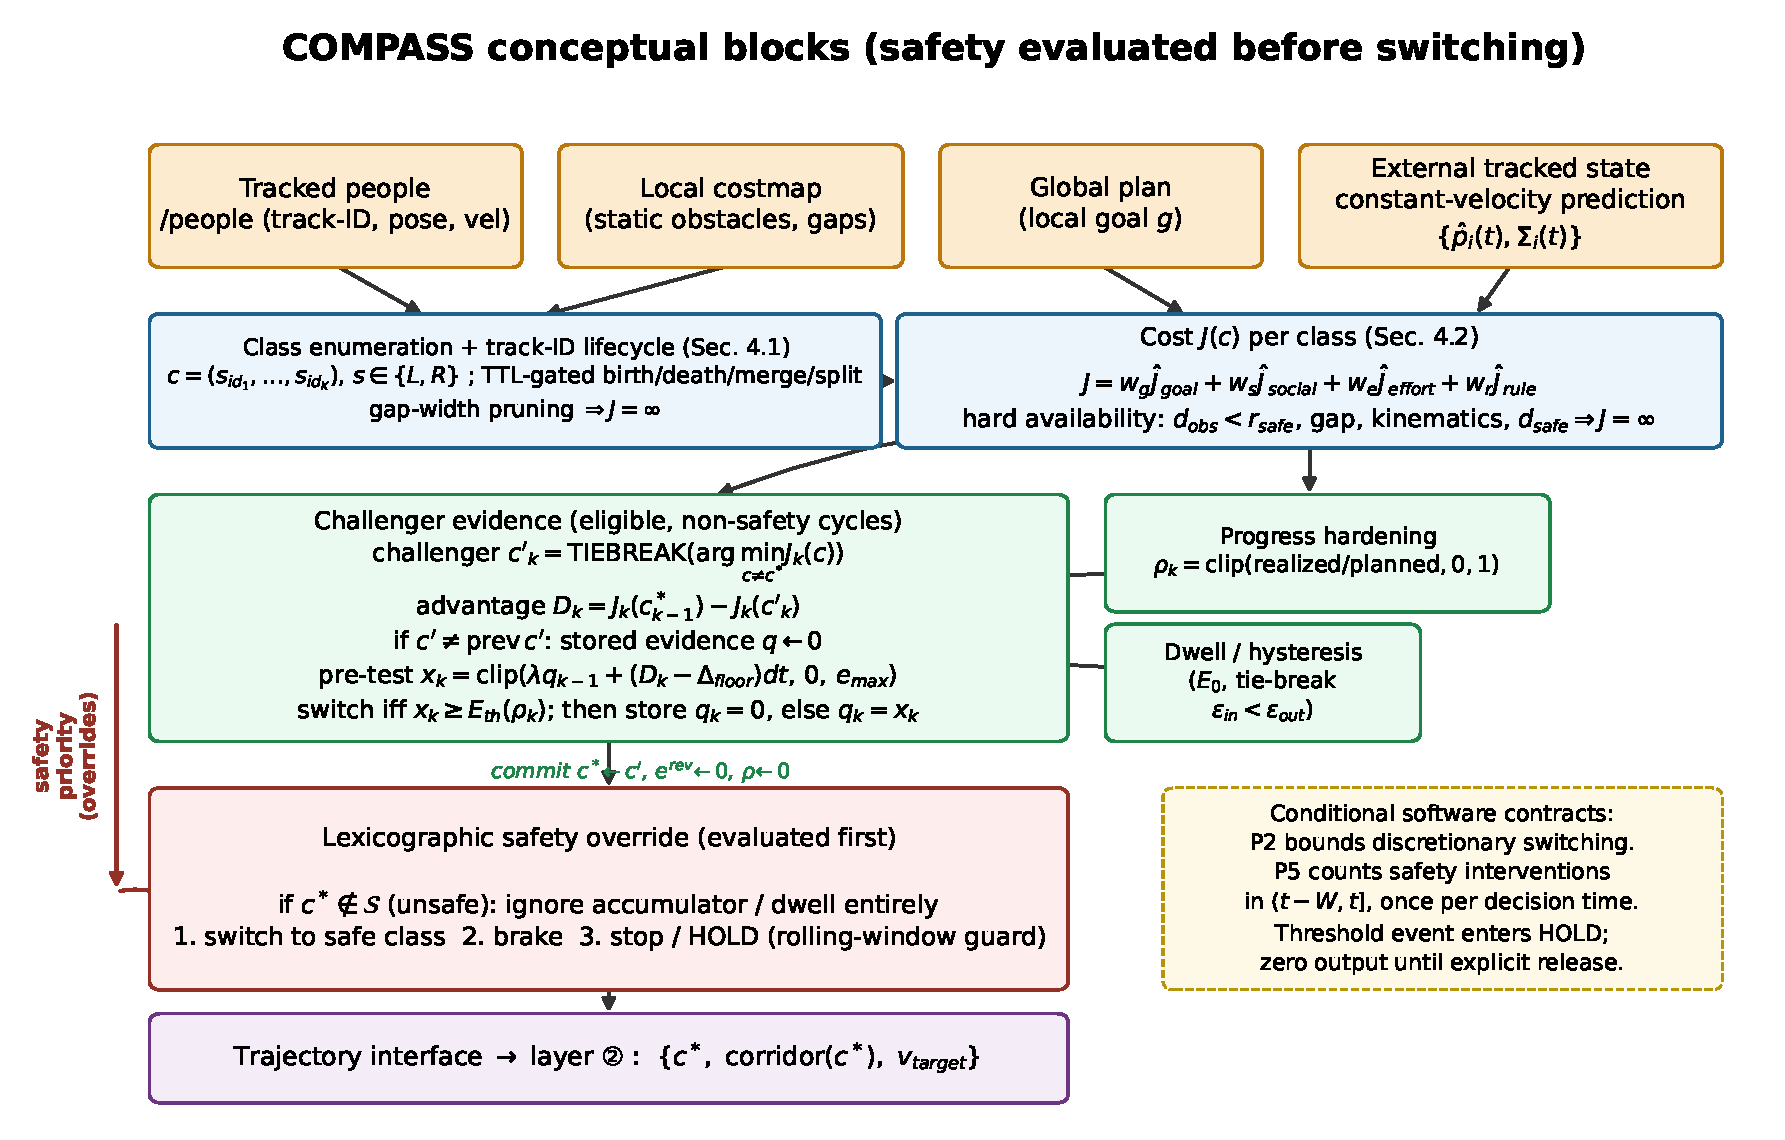
\includegraphics[width=\linewidth]{figures/fig_decision_flow.pdf}
\caption{\textbf{Overview of the \sname\ decision layer.} Conceptual blocks, not a literal execution-order flowchart. Tracked-person, costmap and plan inputs feed class/cost evaluation; safety has priority over discretionary evidence. The diagram distinguishes pre-test evidence $x$ from stored post-reset evidence $q$ and shows P5's conditional rolling-window HOLD contract. The integrated pseudocode (\cref{alg:compass}) specifies the actual control order.}
\label{fig:decisionflow}
\end{figure}


Autonomous serving, delivery, and guide robots are no longer confined to isolated industrial spaces; they now operate in corridors, lobbies, and sidewalks where people move freely. The central difficulty of such shared spaces is not static-obstacle avoidance but \emph{interactive passing decisions} with people who continuously change position and intent. In narrow-corridor head-on encounters, situations where the robot overtakes a person or a person overtakes the robot, and crossing-style traversals, the robot must continually judge ``which side to pass on, whether to proceed or yield, whether to stop.''

Widely used local planners (the \texttt{DWA} family~\citep{fox1997dwa}, \texttt{MPPI}~\citep{williams2017mppi}, \texttt{TEB}~\citep{rosmann2017teb}) re-optimize a cost function at every control cycle. This greedy re-optimization is natural in static environments, but in ambiguous configurations where the costs of the two passing directions are similar, minor sensor noise or a small movement by the person alone can flip the choice from one cycle to the next. As a result, the robot dithers side to side (oscillation) or, unable to commit to either side, comes to a stop --- an outcome reminiscent of the freezing robot problem~\citep{trautman2010}, whose original diagnosis is uncertainty growth rather than commitment failure. Oscillation is not only inefficient --- it also prevents people from reading the robot's intent, undermining both safety and trust. Topology-aware planners recognize the problem but address it through a soft topological-invariance cost~\citep{mavrogiannis2023winding}, an implementation-level selection hysteresis~\citep{rosmann2017teb}, or a consistency parameter formalized at the trajectory-optimization layer~\citep{degroot2024topology}; none of these provides an explicit commitment rule at the discrete decision layer together with a provable bound on how often the passing decision may legitimately flip (\cref{sec:related}).

We study insufficient temporal inertia in the passing decision as one mechanism that can contribute to oscillation; this does not exclude perception, prediction, or interaction uncertainty as other causes. To overcome it, we introduce \emph{\sname}, a decision-layer planner that adds explicit temporal consistency to the passing decision itself (\cref{fig:decisionflow}). The intuition mirrors human walking behavior: once a person decides which way to step aside, they tend to hold that direction, changing it only for a clear reason, and stopping immediately when it becomes dangerous. A related intuition --- that committing to a passing direction aids mutual coordination --- appears in the social-navigation literature as social momentum~\citep{mavrogiannis2022momentum}, and \sname\ embodies the ``hold a once-chosen direction'' behavior as an explicit formal rule at the decision layer. Concretely, \sname\ makes three contributions:
\begin{itemize}
\item \emph{ID-Indexed Topological Classes}: By binding the identity of a passing direction to a person's track ID rather than to a flickering geometric gap, we consistently identify ``the corridor chosen last cycle'' at every cycle. The spawning, removal, merging, and splitting of \Class{es} caused by people entering, leaving, clustering, and separating are specified via explicit lifecycle rules and TTLs, as design contracts that the current implementation only partially realizes (\cref{subsec:enum}).
\item \emph{Unified Commitment Switching with Lexicographic Safety}: The switching margin (hysteresis), dwell (persistence), and progress hardening (point of no return) are folded into a single leaky evidence accumulation equation, with safety placed lexicographically above it. Discretionary changes are deliberately slow (``not rushed''), while the safety override is never delayed by commitment inertia (\cref{subsec:switch,subsec:safety}).
\item \emph{Formal Properties with Offline Validation}: We state anti-oscillation (P1), switching-rate bound (P2), safety dominance (P3), maneuver completion (P4), and conditional finite-window escalation to HOLD (P5) as propositions. The load-bearing anti-oscillation guarantee is P2: a deterministic lower bound of $N_{\min} = \lceil \Eth(\rho)/((D_{\max}-\Dfloor)\,dt)\rceil$ control cycles on the interval between consecutive discretionary switches for fixed $dt$ and zero post-switch evidence, holding on every sample path under the range bound $D_k \le D_{\max}$ that the $[0,1]$ cost normalization of \cref{subsec:cost} supplies by construction, and informative under the declared design condition $E_0 > (D_{\max}-\Dfloor)\,dt$ ($N_{\min} \ge 2$; \cref{rem:p2nonvac}). Because P2 is an upper bound on the switching rate and says nothing about switches occurring, we pair it with a conditional response-time bound (\cref{prop:p2live}): the finite deadline applies only while the same challenger remains selected and eligible, updates proceed without reset or HOLD, its advantage stays above the stated lower bound, and the clip/leak equilibrium has sufficient threshold headroom. P1 refines this, for i.i.d.\ challenger advantages, to an exponentially small per-cycle switching probability and per-unit-time switching rate, proved via Lindley domination and Kingman's bound, with the exponent given by the exact Lundberg root $\theta^*$ of the increment law (the closed form $\theta^* \approx 2\Dfloor/(\sigma_D^2\,dt)$ is retained as tuning guidance only); the exponential form is conditional on that independence hypothesis (\cref{subsec:props}). P4 is proven, on top of the progress $\rho$ dynamics and a lower bound on the lateral progress rate, via a reachable-upper-bound containment condition on the challenger accumulator $\Erev$. Verification is split into two tiers. The decision layer's behavioral consistency, a decision-stream observer statistic, and cyclic latency are \emph{measured} using an offline harness that drives the actual decision core (\cref{sec:exp}); performance metrics requiring physical simulation or a real robot, along with external baselines and user studies, are left as planned evaluations (\cref{app:planned}) specified via a pre-registered protocol.
\end{itemize}

We evaluate \sname\ in an offline harness that drives the actual decision core over 5 reproducible encounter scenarios $\times$ 50 seeds against internal comparators and knob ablations. In the ambiguous-tie scenario, the immediate-argmin comparator changes its decision 98.16 times per 10~s encounter on average, whereas \sname\ keeps its commitment with zero changes; across all 250 trials \sname\ averages 0.40 decision changes per encounter against 29.74 for argmin, and no trial exceeds one change (\cref{tab:main,tab:scenario}). The ablations also correct a prior hypothesis: removing the hysteresis margin or progress hardening alone produces no observed regression in this regime, so the leaky accumulator itself is the primary oscillation-suppression mechanism. A historical decision-core-only timing run gives p99 $58.6\,\mu$s and max $651.3\,\mu$s at $K=3$ (8 classes), about $1.30\%$ of a 20~Hz period. These results establish the conditional decision rule and its offline behavioral consistency; they do not measure physical safety, human-perceived legibility, or comparison against external planners, which remain the pre-registered next step.
